A continuación, se describen los resultados obtenidos del proceso de detección de temas tendencia, con base en el procedimiento previamente descrito para cada uno de los idiomas seleccionados.

\subsection{Inglés}

Para seleccionar el número de \textit{clusters} a tener en cuenta se obtuvieron las gráficas de la distribución utilizando dos, tres, cuatro y cinco grupos (\textit{véase fig \ref{fig:en_kmeans}}). Vale la pena aclarar que estas gráficas solo presentan una proyección en dos dimensiones del verdadero espacio de 32 dimensiones y se obtuvieron con un análisis de componentes principales (o PCA por sus siglas en inglés). Para el idioma inglés se obtuvieron clusters separados (al menos a un nivel visual) para hasta 4 clusters. Ya al momento de buscar 5 clusters se empezaron a sobreponer las agrupaciones de datos. No obstante, para la selección del parámetro \textit{K} también se tuvo en cuenta las palabras claves o \textit{keywords} obtenidas. \\

\begin{figure}
     \centering
     \begin{subfigure}[b]{0.4\textwidth}
         \centering
         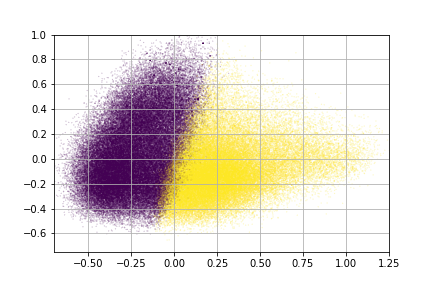
\includegraphics[width=\textwidth]{results/TopicDetection/en/PCA_2.png}
         \caption{2 clusters}
         \label{fig:es_kmeans_2}
     \end{subfigure}
     \hfill
     \begin{subfigure}[b]{0.4\textwidth}
         \centering
         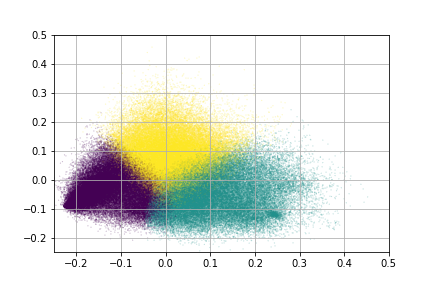
\includegraphics[width=\textwidth]{results/TopicDetection/en/PCA_3.png}
         \caption{3 clusters}
         \label{fig:es_kmeans_3}
     \end{subfigure}
     \hfill
     \begin{subfigure}[b]{0.4\textwidth}
         \centering
         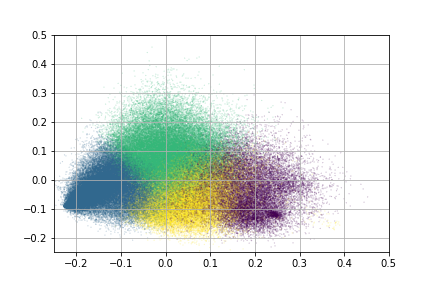
\includegraphics[width=\textwidth]{results/TopicDetection/en/PCA_4.png}
         \caption{4 clusters}
         \label{fig:es_kmeans_4}
     \end{subfigure}
     \hfill
     \begin{subfigure}[b]{0.4\textwidth}
         \centering
         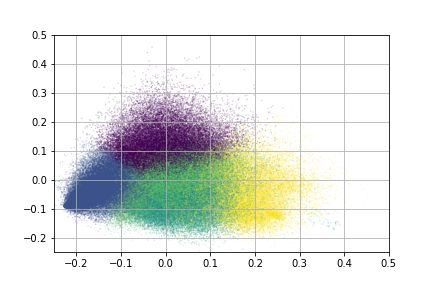
\includegraphics[width=\textwidth]{results/TopicDetection/en/PCA_5.png}
         \caption{5 clusters}
         \label{fig:es_kmeans_5}
     \end{subfigure}
        \caption{Clusters obtenidos con el algoritmo de K-means para diferentes Ks proyectados en un plano 2D utilizando PCA (Inglés)}
        \label{fig:en_kmeans}
\end{figure}

En la figura \ref{fig:en_clusters} se pueden observar las más frecuentes de los documentos más representativos (más cercanos al centro) de cada \textit{cluster}. Con un $K = 3$ se puede evidenciar una clara tendencia en el tipo de clusters obtenidos. En general estos tres \textit{clusters} se pueden asociar a tres momentos temporales distintos que ha vivido la pandemia. Por un lado, en el primer cluster, se pueden observar palabras asociadas a lo que podría ser la aparición del virus con palabras como China y Trump (antiguo presidente de estados unidos) siendo tendencia. Por otro lado, el último cluster hace referencia a palabras que hablan sobre todo el creciente debate acerca de la pandemia, incluyendo el uso o no de tapabocas y de pensar en como manejar la pandemia, ya en este caso aparece la mención a las vacunas. Y, finalmente, en el segundo cluster, se obtienen una mayor presencia de las palabras asociadas a la vacunación  (\textit{vaccine} y \textit{vaccines}), con todavía importancia a palabras relacionadas al uso de tapabocas.

\begin{figure}
    \centering
    \begin{subfigure}[b]{0.49\textwidth}
        \centering
        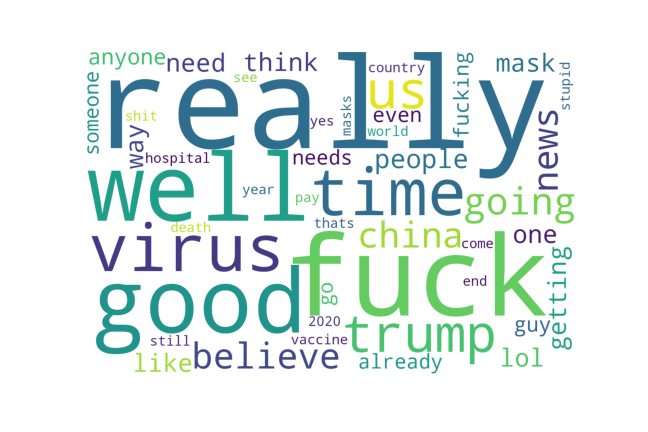
\includegraphics[width=\textwidth]{results/TopicDetection/en/cluster0.png}
        \caption{Cluster 0}
        \label{fig:en_c0}
    \end{subfigure}
    \hfill
    \begin{subfigure}[b]{0.49\textwidth}
        \centering
        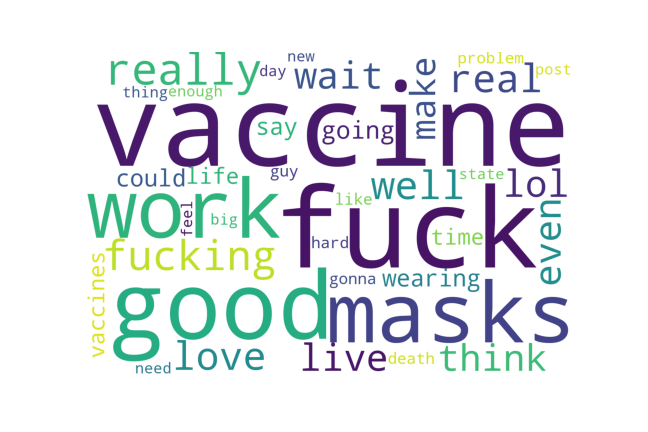
\includegraphics[width=\textwidth]{results/TopicDetection/en/cluster2.png}
        \caption{Cluster 1}
        \label{fig:en_c1}
    \end{subfigure}
    \hfill
    \begin{subfigure}[b]{0.49\textwidth}
        \centering
        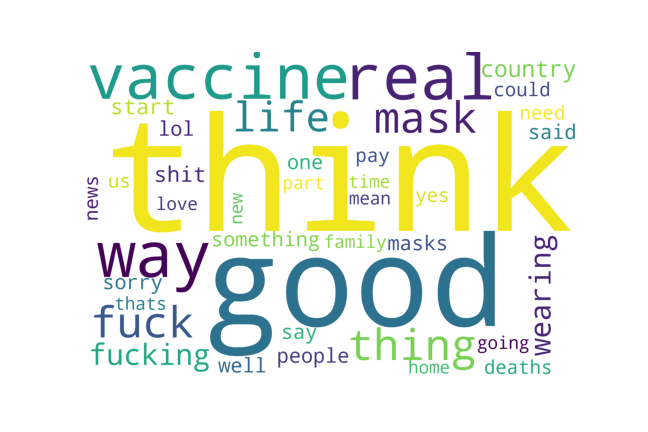
\includegraphics[width=\textwidth]{results/TopicDetection/en/cluster1.png}
        \caption{Cluster 2}
        \label{fig:en_c1}
    \end{subfigure}
    \caption{Palabras más frecuentes en los documentos en el centros de cada uno de los \textit{clusters} (Inglés)}
    \label{fig:en_clusters}
\end{figure}

Las agrupaciones de documentos (o tópicos) obtenidos tienen aún más sentido a nivel temporal cuando se analiza su distribución a través del tiempo. En la figura \ref{fig:en_time} se puede observar la distribución de documentos para los distintos meses de la pandemia. Vale la pena aclarar que se hizo una normalización de los documentos asociados a cada \textit{cluster} sobre cada mes. Esto para evitar que el sesgo de la cantidad de datos recuperados en cada fecha influenciará la representación en la gráfica. Así las cosas se observa que los temas relacionados con el primer cluster (virus, china, trump, etc.) han caído en los últimos meses, mientras que los temas asociados con el segundo cluster (vacunas, vacunación, trabajo) han aumentado en los últimos meses. Mientras tanto la discusión acerca de las mascarillas y el pensamiento correcto de manejar la pandemia se ha mantenido relativamente estable.

\begin{figure}
    \centering
    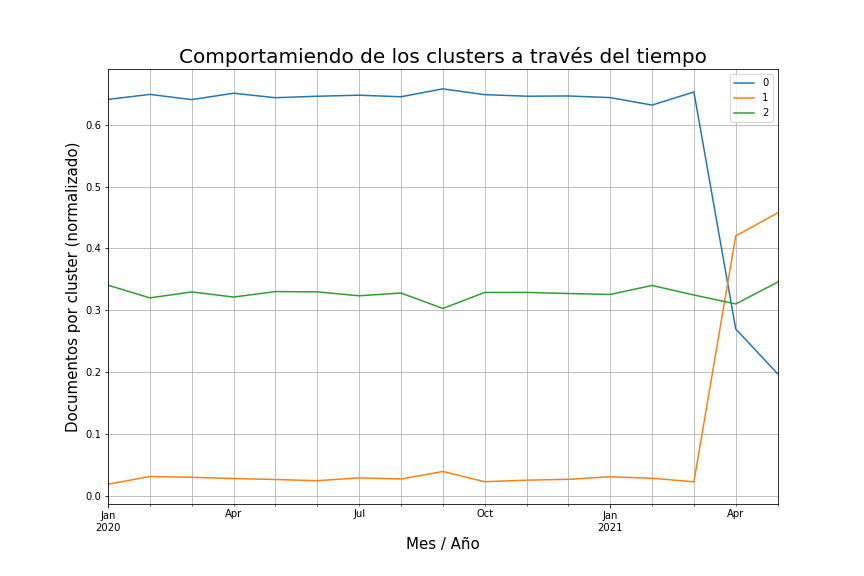
\includegraphics[width=0.9\textwidth]{results/TopicDetection/en/cluster_over_time.png}
    \caption{Comportamiento de los clusters en el tiempo}
    \label{fig:en_time}
\end{figure}


\subsection{Español}

Para seleccionar el número de \textit{clusters} a tener en cuenta se obtuvieron las gráficas de la distribución utilizando dos, tres, cuatro y cinco grupos (\textit{véase fig \ref{fig:es_kmeans}}). La separación de los primeros tres valores (2, 3, y 4) es relativamente clara y se pueden distinguir los colores de cada uno de los grupos. Sin embargo, la distribución obtenida con cinco no permite distinguir claramente el color del quinto \textit{cluster} (\textit{véase fig \ref{fig:es_kmeans_5}}). Por otra parte, si bien es cierto que la separación para dos y tres grupos (\textit{véase fig \ref{fig:es_kmeans_2} y \ref{fig:es_kmeans_3}}) es muy clara y se ve bien distribuida, las tendencias de palabras principales y tiempo no permitían hacer un análisis claro; razón por la cual se decidió trabajar con cuatro grupos.\\

En la figura \ref{fig:es_clusters} se pueden ver las palabras con mayor frecuencia en cada uno de los \textit{clusters}. Respecto al \textit{cluster 0} se percibe cierta tendencia al inicio de la pandemia, momento en el que se empezaba a dialogar sobre la salud, contagios, trabajo y a especular sobre vacunas, conclusión respaldada por la gráfica de análisis temporal (\textit{véase fig \ref{fig:es_time}}) donde se evidencia que un alto porcentaje de documentos en los primeros meses de la pandemia pertenecen a este grupo. A medida que los meses avanzan la participación del \textit{cluster} se reduce un poco, pero sin dejar de ser importante.\\

Con relación al \textit{cluster 1}, la figura \ref{fig:es_c2} da una idea de novedades, nuevos contagios, pacientes, semana a semana, siento la salud un tema aún importante. La figura \ref{fig:es_time} muestra que este \textit{cluster} tiene una importancia relativamente baja pero constante a lo largo de todo el tiempo de pandemia, lo cual podría explicarse teniendo en cuenta que la información sobre novedades está fluyendo constantemente, sin tomar protagonismo del todo.\\

En los últimos dos \textit{clusters} se evidencia casi de inmediato una palabra que viene cobrando importancia desde hace algunos meses para acá: vacunas. Desde el comienzo de la pandemia se hablaba del tema, esperando con ansias información al respecto, pero desde que se iniciaron ensayos en humanos por parte de las farmacéuticas más importantes del mundo el tema ha sido tendencia. Se puede observar un pico en la importancia de estos \textit{clusters} hacia la mitad de 2020. Adicionalmente, en el \textit{cluster 2} se perciben aún temas como muertos, trabajo, salud, con menor importancia, que, como lo respalda la gráfica de temporalidad, han sido tendencia media pero constante durante toda la pandemia. El \textit{cluster 3} indica conversaciones sobre país, mundo, dinero, entre otros.

\begin{figure}
     \centering
     \begin{subfigure}[b]{0.4\textwidth}
         \centering
         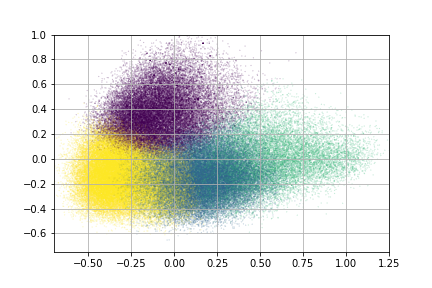
\includegraphics[width=\textwidth]{results/TopicDetection/es/PCA_2.png}
         \caption{2 clusters}
         \label{fig:es_kmeans_2}
     \end{subfigure}
     \hfill
     \begin{subfigure}[b]{0.4\textwidth}
         \centering
         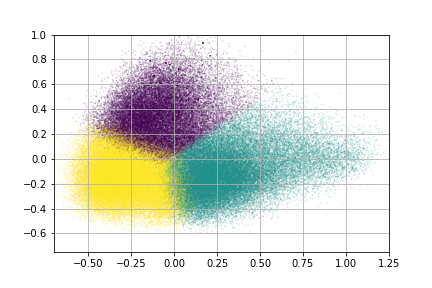
\includegraphics[width=\textwidth]{results/TopicDetection/es/PCA_3.png}
         \caption{3 clusters}
         \label{fig:es_kmeans_3}
     \end{subfigure}
     \hfill
     \begin{subfigure}[b]{0.4\textwidth}
         \centering
         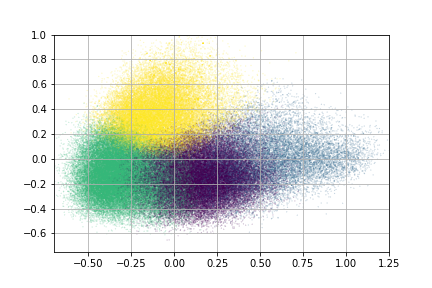
\includegraphics[width=\textwidth]{results/TopicDetection/es/PCA_4.png}
         \caption{4 clusters}
         \label{fig:es_kmeans_4}
     \end{subfigure}
     \hfill
     \begin{subfigure}[b]{0.4\textwidth}
         \centering
         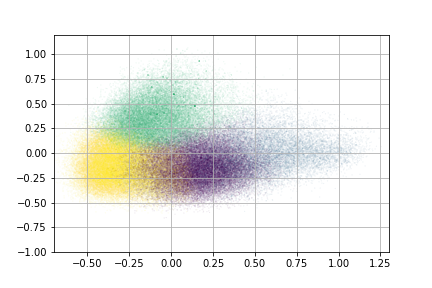
\includegraphics[width=\textwidth]{results/TopicDetection/es/PCA_5.png}
         \caption{5 clusters}
         \label{fig:es_kmeans_5}
     \end{subfigure}
        \caption{Resultados de K-means con diferente número de clusters}
        \label{fig:es_kmeans}
\end{figure}



\begin{figure}
    \centering
    \begin{subfigure}[b]{0.49\textwidth}
        \centering
        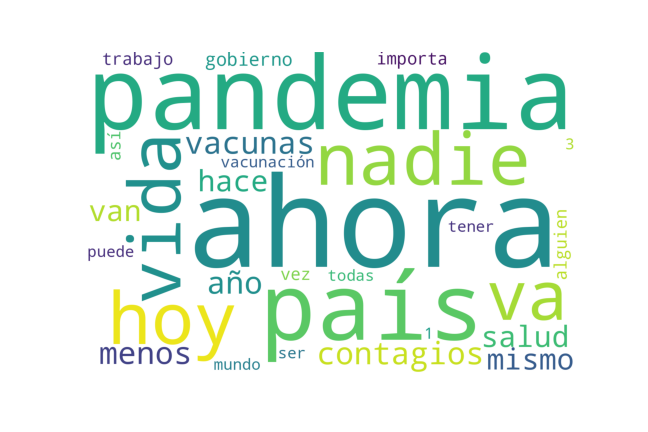
\includegraphics[width=\textwidth]{results/TopicDetection/es/cluster0.png}
        \caption{Cluster 0}
        \label{fig:es_c0}
    \end{subfigure}
    \hfill
    \begin{subfigure}[b]{0.49\textwidth}
        \centering
        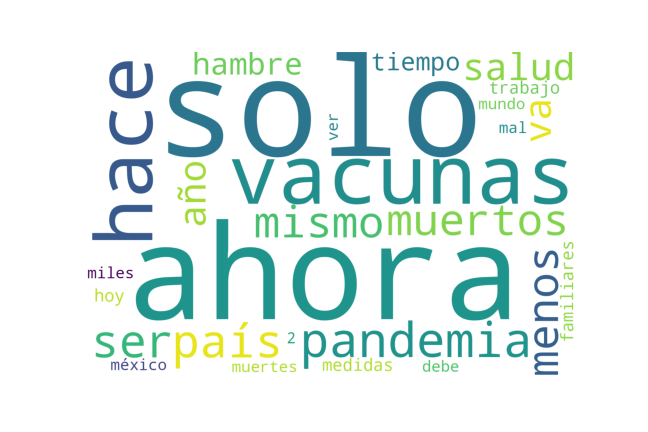
\includegraphics[width=\textwidth]{results/TopicDetection/es/cluster1.png}
        \caption{Cluster 1}
        \label{fig:es_c1}
    \end{subfigure}
    \hfill
    \begin{subfigure}[b]{0.49\textwidth}
        \centering
        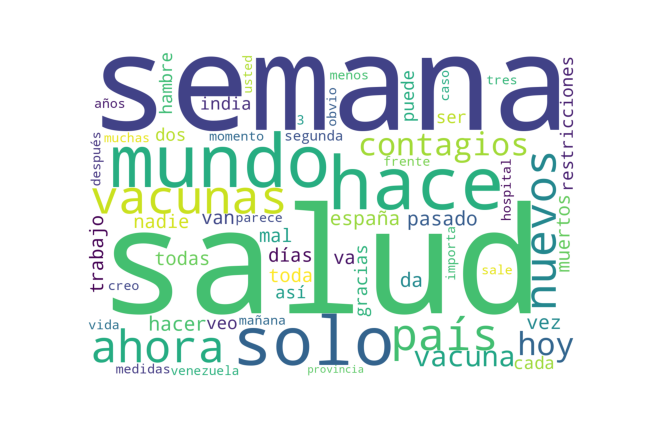
\includegraphics[width=\textwidth]{results/TopicDetection/es/cluster2.png}
        \caption{Cluster 2}
        \label{fig:es_c2}
    \end{subfigure}
    \hfill
    \begin{subfigure}[b]{0.49\textwidth}
        \centering
        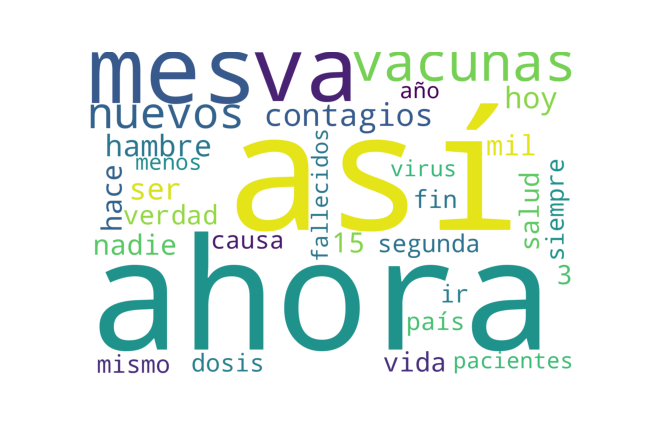
\includegraphics[width=\textwidth]{results/TopicDetection/es/cluster3.png}
        \caption{Cluster 3}
        \label{fig:es_c3}
    \end{subfigure}
    \caption{Principales palabras de cada uno de los clusters}
    \label{fig:es_clusters}
\end{figure}

\begin{figure}
    \centering
    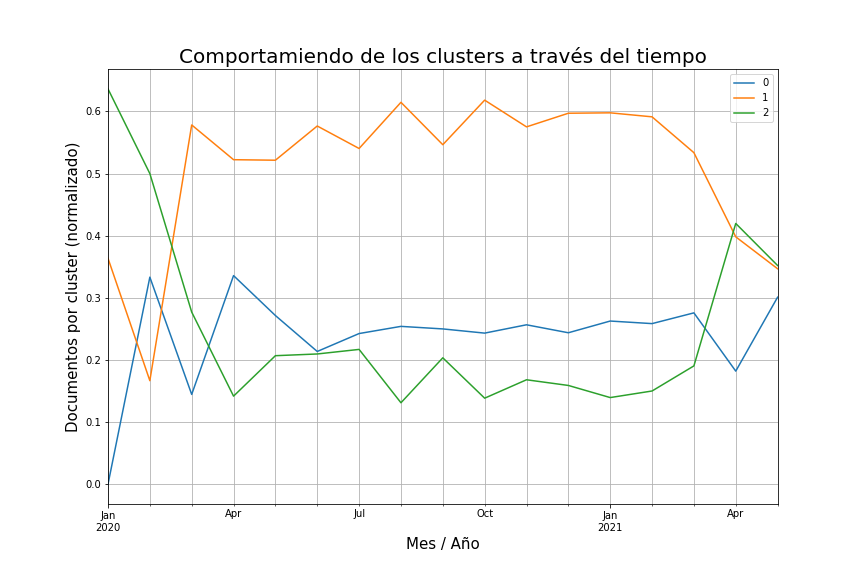
\includegraphics[width=0.9\textwidth]{results/TopicDetection/es/cluster_over_time.png}
    \caption{Comportamiento de los clusters en el tiempo}
    \label{fig:es_time}
\end{figure}

\subsection{Francés}